\documentclass[tikz,border=2pt]{standalone}
\usepackage{amsmath}
\usepackage{pgfplots}
\pgfplotsset{compat=1.18}

\begin{document}
% arcsin and arccos live on [-1,1] (left); arctan is defined on all of R and is squeezed between
% the horizontal asymptotes y = ±π/2 (right).
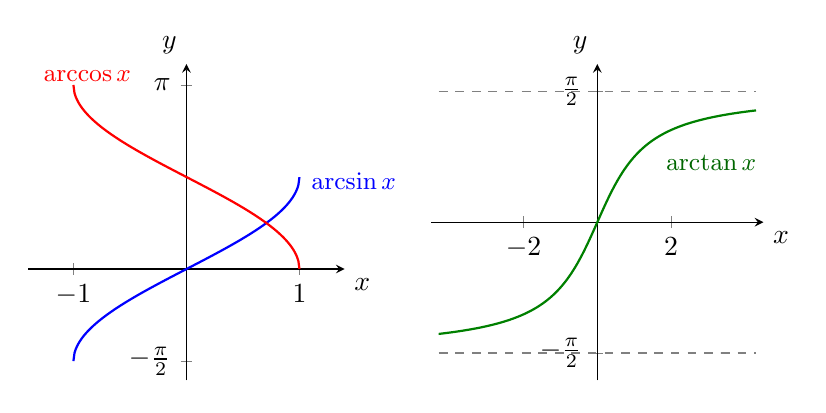
\begin{tikzpicture}
	\begin{axis}[
		name=left,
		axis lines=middle,
		xmin=-1.4, xmax=1.4,
		ymin=-1.9, ymax=3.5,
		xtick={-1,1}, ytick={-1.5708,3.1416}, yticklabels={$-\tfrac\pi2$,$\pi$},
		xlabel={$x$}, ylabel={$y$},
		xlabel style={below right}, ylabel style={above left},
		samples=200, smooth, clip=false,
		width=5.6cm, height=5.6cm
		]
		\addplot[thick, blue, domain=-1:1] {asin(x)/180*pi};
		\addplot[thick, red, domain=-1:1] {acos(x)/180*pi};
		\node[blue, anchor=west, font=\small] at (axis cs:1.02,1.5) {$\arcsin x$};
		\node[red, anchor=west, font=\small] at (axis cs:-1.35,3.3) {$\arccos x$};
	\end{axis}
	\begin{axis}[
		at={(left.east)}, anchor=west, xshift=1.1cm,
		axis lines=middle,
		xmin=-4.5, xmax=4.5,
		ymin=-1.9, ymax=1.9,
		xtick={-2,2}, ytick={-1.5708,1.5708}, yticklabels={$-\tfrac\pi2$,$\tfrac\pi2$},
		xlabel={$x$}, ylabel={$y$},
		xlabel style={below right}, ylabel style={above left},
		samples=200, smooth, clip=false,
		width=5.8cm, height=5.6cm
		]
		\addplot[gray, dashed, domain=-4.3:4.3] {1.5708};
		\addplot[gray, dashed, domain=-4.3:4.3] {-1.5708};
		\addplot[thick, green!50!black, domain=-4.3:4.3] {atan(x)/180*pi};
		\node[green!40!black, anchor=south west, font=\small] at (axis cs:1.6,0.5) {$\arctan x$};
	\end{axis}
\end{tikzpicture}
\end{document}
